\documentclass{wissdoc}
% ----------------------------------------------------------------
% student thesis -- main document
% ----------------------------------------------------------------
%%
%%
% wissdoc Options: draft, relaxed, pdf --> see wissdoc.cls
% ------------------------------------------------------------------
% additional packages: (for documentation see "latex <package>.dtx")
\usepackage[numbers,sort&compress]{natbib}

\usepackage[english]{babel} % language settings
\usepackage[utf8]{inputenc} % concrete encoding of symbols
\usepackage[printonlyused]{acronym} % show only acronyms used throughout the document
\usepackage{listings} % source code listings
% packages to allow drawing tikz pictures
\usepackage{pgfplots}
\pgfplotsset{compat=1.7}
\usepackage{tikz}
	\usetikzlibrary{arrows,positioning,backgrounds,fit,trees} 
	\usetikzlibrary{fadings,shapes.geometric}
	\usetikzlibrary{decorations,scopes,calc,decorations.pathreplacing}

% useful packages:
\usepackage{amsmath} % standard package for math stuff
% \usepackage{rotating} % rotation of figures, tables etc.
% \usepackage{enumitem} % cotroll the layout of itemize, enumerate, and description 
% \usepackage{pdfpages} % enables including single pages of a pdf or the whole pdf
% \usepackage{newunicodechar} % re-define unicode characters \newunicodechar{}{}


\usepackage{varioref} 
% \usepackage{verbatim}
% \usepackage{float}    %z.B. \floatstyle{ruled}\restylefloat{figure}
% \usepackage{subfigure}
% \usepackage{fancybox} % cotrolls for boxes (shadows, other forms, etc.) 
\usepackage{tabularx} % automatic resizing of column width in tables
% \usepackage{supertab} % enables tables over multiple pages
\usepackage{booktabs}
%% ---------------- end of usepackages -------------


%% Meta-information of the pdf
\hypersetup{
 pdfauthor={N.N.},
 pdftitle={Not set}
 pdfsubject={Not set},
 pdfkeywords={Not set}
}

% Print URLs not in Typewriter Font
\def\UrlFont{\rm}

\newcommand{\blankpage}{% creates empty page without page numbers, puts the next page right
 \clearpage{\pagestyle{empty}\cleardoublepage}
}

%% options for the whole document

% seperation hints
% important! 
% in ngerman-paket the following seperation hints are included:
% "- = additional seperation point
% "| = Avoidance of ligatures and possible separation (e.g., Schaf"|fell)
% "~ = Hyphen at which no separation is allowed (e.g., bergauf und "~ab)
% "= = Hyphen where words before and after may be separated
% "" = Separation point without generating a hyphen (e.g., und/""oder)

% Describe seperation hints for words here
\hyphenation{
% Pro-to-koll-in-stan-zen
% Ma-na-ge-ment  Netz-werk-ele-men-ten
% Netz-werk Netz-werk-re-ser-vie-rung
% Netz-werk-adap-ter Fein-ju-stier-ung
% Da-ten-strom-spe-zi-fi-ka-tion Pa-ket-rumpf
% Kon-troll-in-stanz
}

% open index file
\ifnotdraft{\makeindex}
%%%%%%%%%%%%%% includeonly %%%%%%%%%%%%%%%%%%%
% Only the parts that are listed here are included!
\includeonly{%
%########## include essentials ###########
essentials/frontpage,%
% A declaration is mandatory in KA for final theses
essentials/declaration,
% It is not mandatory to have an appendix, 
%but most of the time you have some data or additional visuals that do not fit into the thesis
essentials/appendix,
% define acronyms used in this thesis 
% acronyms will be listed in the acronym reference automatically
essentials/acronyms, %
%########## utility includes ###########
% defines colors according to KIT coporate desingn and names them for your convinience
utility/colorScheme,
% use this document to re-define latex commands, so that they will suite your needs
utility/commandReDef,
% define customized environments if required
utility/environmentDef,
% define your own lstlist style.
% For instance to use java or python code highlighting or to have a customized pseudocode style
utility/lststyle,
% Define latex macros, and new commands for your convinience
utility/macros,
% map mathmatical symbols and inline formulas to semantic names
% for instance: mapping the '\wedge' command to teh semantic name '\pand' to use it as symbol for a propositional and
utility/mathSymbolDef,
% Define terms that are used frequently so that they are always spelled the same way
utility/termDef,
% Define custom tikz styles for your thesis, if required
utility/tikzStyle,
% map urls to short hand commands for a convinient use
utility/urls,
%########## include chapters ###########
% Abstract in german
chapters/000_abstract_de,
% Abstract in english
chapters/000_abstract_eng,
% motivation, research goal, structure
chapters/100_introduction,
% problem statement and motivating example
% maybe merged with introduction or basics
chapters/200_problemstatement,
% background and basics to understand your thesis
chapters/300_basics,
% Problembeschreibung (Detail) und Related Work
%chapters/analysis,   
% Description of the problem solution (concepts, general architecture, ...)
chapters/400_design, 
% example chapter showing some latex concepts to use in your thesis
chapters/xxx_example,
% Description of the conversion/implementation
chapters/500_implementation,  
% Description of the evaluation for your concepts (planning, execution, results, discussion)
chapters/600_evaluation,      
% describe related research and describe how your work deffers from what exists
% based on the topic this section may be placed after the basics
chapters/700_relatedwork, 
% Summary of your work and its results.
% Includes a discussion about future work and how to procede with our results
chapters/800_conclusion,  
}
%%%%%%%%%%%%%%%%%%%%%%%%%%%%%%%%%%%%%%%%%%%%%%
\begin{document}
%
%% ++++++++++++++++++++++++++++++++++++++++++
%% including utility files
%% ++++++++++++++++++++++++++++++++++++++++++
% define acronyms used in this thesis 
% defines colors according to KIT coporate desingn and names them for your convinience
%%% Here you define shorthands for colors you want to use
%%-----------------------------------------------%
%% KIT Colors                                    %
%%-----------------------------------------------%

%% KIT Green
\definecolor{kitGreen1}{HTML}{00876c}
\definecolor{kitGreen2}{HTML}{b7fff5}
\definecolor{kitGreen3}{HTML}{6fffec}
\definecolor{kitGreen4}{HTML}{27ffe2}
\definecolor{kitGreen5}{HTML}{007162}
\definecolor{kitGreen6}{HTML}{004b41}
%% =========================================
%% KIT Blue
\definecolor{kitBlue1}{HTML}{4664aa}
\definecolor{kitBlue2}{HTML}{d9dfef}
\definecolor{kitBlue3}{HTML}{b3c0df}
\definecolor{kitBlue4}{HTML}{8ca1d0}
\definecolor{kitBlue5}{HTML}{354b7f}
\definecolor{kitBlue6}{HTML}{233255}
%% =========================================
%% KIT Black
\definecolor{kitBlack1}{HTML}{404040}
\definecolor{kitBlack2}{HTML}{000000}
\definecolor{kitBlack3}{HTML}{7f7f7f}
\definecolor{kitBlack4}{HTML}{595959}
\definecolor{kitBlack5}{HTML}{262626}
\definecolor{kitBlack6}{HTML}{0d0d0d}
%% =========================================
%% KIT May Green
\definecolor{kitMayGreen1}{HTML}{77a200}
\definecolor{kitMayGreen2}{HTML}{e8f2d7}
\definecolor{kitMayGreen3}{HTML}{d2e4ae}
\definecolor{kitMayGreen4}{HTML}{bbd786}
\definecolor{kitMayGreen5}{HTML}{69882d}
\definecolor{kitMayGreen6}{HTML}{465b1e}
%% =========================================
%% KIT Purple
\definecolor{kitPurple1}{HTML}{a3107c}
\definecolor{kitPurple2}{HTML}{f9c3eb}
\definecolor{kitPurple3}{HTML}{f386d6}
\definecolor{kitPurple4}{HTML}{ed4ac2}
\definecolor{kitPurple5}{HTML}{7a0c5d}
\definecolor{kitPurple6}{HTML}{52083e}
%% =========================================
%% KIT Brown
\definecolor{kitBrown1}{HTML}{a7822e}
\definecolor{kitBrown2}{HTML}{df9b1b}
\definecolor{kitBrown3}{HTML}{f9ebd1}
\definecolor{kitBrown4}{HTML}{f4d7a2}
\definecolor{kitBrown5}{HTML}{eec474}
\definecolor{kitBrown6}{HTML}{6f4e0e}
%% =========================================
%% KIT Cyan
\definecolor{kitCyan1}{HTML}{079ede}
\definecolor{kitCyan2}{HTML}{d3ecf9}
\definecolor{kitCyan3}{HTML}{a7d9f3}
\definecolor{kitCyan4}{HTML}{7bc7ec}
\definecolor{kitCyan5}{HTML}{187aaa}
\definecolor{kitCyan6}{HTML}{105172}
%% =========================================
%% KIT Gray
\definecolor{kitGray1}{HTML}{d9d9d9}
\definecolor{kitGray2}{HTML}{c3c3c3}
\definecolor{kitGray3}{HTML}{a3a3a3}
\definecolor{kitGray4}{HTML}{6d6d6d}
\definecolor{kitGray5}{HTML}{363636}
\definecolor{kitGray6}{HTML}{161616}
%% =========================================
%% KIT Yellow
\definecolor{kitYellow1}{HTML}{fce500}
\definecolor{kitYellow2}{HTML}{fffacb}
\definecolor{kitYellow3}{HTML}{fff698}
\definecolor{kitYellow4}{HTML}{fff164}
\definecolor{kitYellow5}{HTML}{bdac00}
\definecolor{kitYellow6}{HTML}{7e7200}
%% =========================================
%% KIT White
\definecolor{kitWhite1}{HTML}{ffffff}
\definecolor{kitWhite2}{HTML}{f2f2f2}
\definecolor{kitWhite3}{HTML}{d9d9d9}
\definecolor{kitWhite4}{HTML}{bfbfbf}
\definecolor{kitWhite5}{HTML}{a6a6a6}
\definecolor{kitWhite6}{HTML}{7f7f7f}

%%-----------------------------------------------%
%% Colors for special commands                   %
%%-----------------------------------------------%
% color for background
\definecolor{background}{named}{white}
% color for background borders
\definecolor{bgborder}{named}{black}
% color for comments 
\definecolor{comment}{named}{kitPurple1}
% color for hints shown in this thesis template.
\definecolor{hint}{named}{kitBlue1}
% color for pdf links
\definecolor{pdflinkcolor}{named}{kitMayGreen1}
% color for pdf links
\definecolor{pdfcitecolor}{named}{kitCyan1}
% color for todos
\definecolor{todo}{named}{kitPurple1}

% use this document to re-define latex commands, so that they will suite your needs
%% Here you can re-define latex commands to suite your requirements
% define customized environments if required
%% Here you define environments to use in your thesis
%% That also includes the definition of environments such as mathmatical theorems, defintions etc.

%=============================
% normal environments        =
%=============================

%Example Environment
%\newcounter{EXAMPLE}[section]
%\newenvironment{EXAMPLE}
%% begin env
%{\refstepcounter{EXAMPLE}\par\medskip
%	\noindent \textbf{\textit{Example~\thesection.\theEXAMPLE}} 
%	\begin{itshape}	
%}
%%end Env
%{\end{itshape}
%}
%\newcommand{\EXAMRef}[1]{\color{black} Example~\ref{#1}\color{black}}

%% environment to mark changed parts of the paper
\newenvironment{ChangedEnv}{
	\color{green3}
}
{\color{black} \vspace{0.3cm}
}

%===========================================
% mathematical definitions and theorems    =
%===========================================
%\newtheorem{definition}{Definition}[chapter]
\newtheorem{theorem}{Theorem}[chapter]
\newtheorem{lemma}{Lemma}[chapter]
% define your own lstlist style.
% For instance to use java or python code highlighting or to have a customized pseudocode style
%% Here you can define various lstlisting styles to make your source code listings look pretty.

\lstdefinestyle{java}{
%code formatting
	language=Java,
	tabsize=4,
	breaklines=false,
	basicstyle=\fontfamily{pcr}\footnotesize\selectfont,
	commentstyle=\fontshape{it}\color{darkgray}\selectfont,
	keywordstyle=\fontseries{b}\selectfont,
	stringstyle=\fontfamily{cmr}\selectfont,
%line numbering
	numbers=left,
	numberstyle=\footnotesize,
%frame properties
	captionpos=b,
	frame=single,%trblTRBL
	framesep=3pt,
	xleftmargin=4pt,
	xrightmargin=4pt,
	rulecolor=\color{bgborder},
}
% Define latex macros, and new commands for your convinience
%% Here you define commands for convienience 

% command to mark todos for yourself
\newcommand{\todo}[1]{{\color{todo} #1}}

% command to indicate missing content as todo
\newcommand{\todots}{\todo{\ldots}}

 % macro to define hints as guidelines for content and structure. 
 % All hints must be removed in the final version of your thesis
\newcommand{\hint}[1]{{\color{hint}\textit{#1}}}

% map mathmatical symbols and inline formulas to semantic names
% for instance: mapping the '\wedge' command to teh semantic name '\pand' to use it as symbol for a propositional and
%% Here you define shorthands for mathmatical symbol and definitions to use throughout your thesis.

%=============================================
% propositional formulas
%=============================================
\newcommand{\pand}{\wedge}
\newcommand{\por}{\vee}
\newcommand{\pnot}{\neg}
\newcommand{\pequals}{\Leftrightarrow}
\newcommand{\pimplies}{\Rightarrow}
\newcommand{\pnimplies}{\nRightarrow}
\newcommand{\patmostone}{\mbox{\textit{atmost1}}}
\newcommand{\pchooseone}{\mbox{\textit{choose1}}}


% Define terms that are used frequently so that they are always spelled the same way
%% this is the place to define commands for important terms of the paper
%% Definition of mathmatical terms --> usage in text requires math environment
%=========================
%% feature model
%=========================
\newcommand{\model}{\mathcal{M}}

%=========================
%% Feature space
%=========================
\newcommand{\featureSpaceLHS}{\mathcal{F}}
\newcommand{\featureSpaceRHS}{\{f_0, f_1, \dots, f_o\}}
\newcommand{\featureI}{f_i}
\newcommand{\featureSpaceCount}{o}

%=========================
%% dependencie space
%=========================
\newcommand{\depSpaceLHS}{\mathcal{D}}
\newcommand{\depSpaceRHS}{\{d_0, d_1, \dots, d_p\}}
\newcommand{\depSpaceI}{d_i}
\newcommand{\depSpaceCount}{p}

%=========================
%% Literals of model
%=========================
\newcommand{\litSpaceLHS}{\mathcal{L}(\model)}
\newcommand{\litSpace}{\mathcal{L}}
\newcommand{\literal}{f}
\newcommand{\litI}{\literal_i}
\newcommand{\litN}{n}
\newcommand{\litSpaceRHS}{\setOpen \literal_{0}, \literal_{1}, \dots, \literal_{n} \bigPipe \litN \in \abs{\featureSpaceLHS} \setClose}

%=========================
%% t-wise interaction size (t=2, t=3 usw.)
%=========================
\newcommand{\twise}{t}

%=========================
%% feature interaction formula
%=========================
\newcommand{\interactionLHS}{(f_{1} \dots f_{t})}
\newcommand{\featurePermutation}{2^{\featureSpaceLHS}}

%=========================
%% Configuration space
%=========================
\newcommand{\confSpace}{\mathcal{C}}

%=========================
%% configuration 
%=========================
\newcommand{\conf}{C}

%=========================
%% sample 
%=========================
\newcommand{\samp}{S}

% Define custom tikz styles for your thesis, if required
%% Here you define tikzstyles to use

%=========================
%Pie chart
%=========================
\newcommand{\slice}[4]{
  \pgfmathparse{0.5*#1+0.5*#2}
  \let\midangle\pgfmathresult

  % slice
  \draw[thick,
	%fill=background
	] (0,0) -- (#1:1) arc (#1:#2:1) -- cycle;

  % outer label
  \node[label=\midangle:#4] at (\midangle:1) {};

  % inner label
  \pgfmathparse{min((#2-#1-10)/110*(-0.3),0)}
  \let\temp\pgfmathresult
  \pgfmathparse{max(\temp,-0.5) + 0.8}
  \let\innerpos\pgfmathresult
  \node at (\midangle:\innerpos) {#3};
}
\newcommand{\mypiechart}[2]{
	\begin{tikzpicture}[scale=#1]
		\newcounter{a}
		\newcounter{b}
		\foreach \p/\t in {#2}
			{
				\setcounter{a}{\value{b}}
				\addtocounter{b}{\p}
				\slice{\thea/100*360}
							{\theb/100*360}
							{\p\%}{\t}
			}
	\end{tikzpicture}
}
% map urls to short hand commands for a convinient use
%% Here you can define shorthands for urls you want to use throughout your thesis

\urldef{\busyboxdata}\url{https://github.com/TUBS-ISF/busybox-case_study}
\urldef{\solettadata}\url{https://github.com/TUBS-ISF/soletta-case-study}
\urldef{\toyboxdata}\url{https://github.com/TUBS-ISF/toybox-case-study}
\urldef{\uclibcdata}\url{https://github.com/TUBS-ISF/uclibc-case-study}
\urldef{\fiascodata}\url{https://github.com/TUBS-ISF/fiasco-case-study}

\urldef{\busyboxLink}\url{https://www.busybox.net/}
\urldef{\solettaLink}\url{https://github.com/solettaproject/soletta}
\urldef{\toyboxLink}\url{https://github.com/landley/toybox}
\urldef{\uclibcLink}\url{https://github.com/wbx-github/uclibc-ng/}
\urldef{\fiascoLink}\url{https://github.com/kernkonzept/fiasco}

\urldef{\tva}\url{https://tva.kastel.kit.edu/}
%
%% ++++++++++++++++++++++++++++++++++++++++++
%% Frontmatter
%% ++++++++++++++++++++++++++++++++++++++++++
\frontmatter
\pagenumbering{roman}
\ifnotdraft{
 %% Titelseite

\def\usesf{}
\let\usesf\sffamily % comment out this line for normal TeX font

\newsavebox{\Reviewer}
\savebox{\Reviewer}{\usesf Prof.~Dr.}
\newsavebox{\SecondReviewer}
\savebox{\SecondReviewer}{\usesf Prof.~Dr.}

\begin{titlepage}
\setlength{\unitlength}{1pt}
\begin{picture}(0,0)(85,770)

\includegraphics[width=\paperwidth]{logos/KIT_Deckblatt}
\end{picture}

%\vspace*{-39pt}\hspace*{300pt}\includegraphics[width=.27\paperwidth]{logos/IOSB}
\vspace*{-39pt}\hspace*{368pt}
\includegraphics[width=.15\paperwidth]{logos/LogoTaglineEnglishColor.pdf}

\thispagestyle{empty}

%\begin{titlepage}
%%\let\footnotesize\small \let\footnoterule\relax
\begin{center}
\hbox{}
\vfill
{\usesf
{\huge\bfseries Title of the Thesis \\ \par}
\vskip 1.8cm
Bachelor's Thesis\\
of\\[2mm]
\vskip 1cm

{\large\bfseries Name Surname\\}
\vskip 1.2cm
at the Department of Informatics\\
Institute of Information Security and Dependability\\
Test, Validation and Analysis (TVA)
\vskip 3cm
\begin{tabular}{p{5.5cm}l}
Reviewer: & \usebox{\Reviewer} \\
Second Reviewer: & \usebox{\SecondReviewer} \\
Advisors: &  M.Sc. \\
 & Dr. 
\end{tabular}
\vskip 3cm
Completion period:\qquad ??.~Month~2023 -- ??.~Month~2023
}
\end{center}
\vfill
\end{titlepage}
%% End of titlepage


%%% Local Variables: 
%%% mode: latex
%%% TeX-master: "thesis"
%%% End: 

 \blankpage % empty page for title backsite
 %
 % The following declaration is mandatory for diploma theses
 % (see examination regulations), not required for student research projects
 \thispagestyle{empty}
\vspace*{32\baselineskip}
\hbox to \textwidth{\hrulefill}
\par
Ich versichere wahrheitsgemäß, die Arbeit selbstständig verfasst, alle benutzten Hilfsmittel vollständig und genau angegeben und alles kenntlich gemacht zu haben, was aus Arbeiten anderer unverändert oder mit Abänderungen entnommen wurde sowie die Satzung des KIT zur Sicherung guter wissenschaftlicher Praxis in der jeweils gültigen Fassung beachtet zu haben.
%Ich erkläre hiermit, dass ich die vorliegende Arbeit selbständig verfasst und
%keine anderen als die angegebenen Quellen und Hilfsmittel benutzt, 
%die wörtlich oder inhaltlich übernommenen Stellen als solche kenntlich 
%gemacht und die Satzung des KIT zur Sicherung guter wissenschaftlicher 
%Praxis in der jeweils gültigen Fassung beachtet habe.
\vspace*{2cm}
\\Karlsruhe, den ??. ?????? 2023\hfill \hbox to 8cm{\hrulefill}

%%%%%%%%%%%%%%%%%%%%%%%%%%%%%%%%%%%%%%%%%%%%%%%%%%%%%%%%%%%%%%%%%%%%%%%%
%% Hinweis:
%%
%% Diese Erklärung wird von der Prüfungsordnung für Diplom-, Master,
%% und Bachelorarbeiten verlangt und ist zu unterschreiben. 
%% Für Studienarbeiten ist diese Erklärung nicht zwingend notwendig, 
%% schadet aber auch nicht.
%%%%%%%%%%%%%%%%%%%%%%%%%%%%%%%%%%%%%%%%%%%%%%%%%%%%%%%%%%%%%%%%%%%%%%%%
\clearpage







 \blankpage % Blank page on declaration back
}
%
%% *************** Start of chapters ****************
\chapter*{Zusammenfassung}
% This is the abstract in german
\hint{Neben dem Titel ist die Zusammenfassung der wichtigste Teil Ihrer Arbeit, da die meisten Leser nur den Titel und die Zusammenfassung lesen werden. Ihr Ziel ist es, den Rest der Arbeit für potenzielle Leser zu bewerben. Dazu erklären Sie kurz, worauf Sie sich in der Arbeit konzentrieren. Mit einer irreführenden Zusammenfassung verpassen Sie interessierte Leser und locken vielleicht sogar Leser mit falschen Annahmen über Ihre Arbeit an, die dann bald aufhören zu lesen. Die Zusammenfassung sollte sowohl das allgemeine Gebiet als auch die interessantesten Erkenntnisse der Arbeit beschreiben. Es ist entscheidend, das richtige Maß an Abstraktion und Länge zu finden. Eine Zusammenfassung besteht in der Regel aus einem Absatz, der deutlich kürzer ist als die Einleitung.}

\hint{Kurzfassungen folgen in der Regel dem gleichen Aufbau. Sie beginnen mit der Beschreibung des Forschungsgebiets sowie des allgemeinen und des spezifischen Problems, auf das Sie sich konzentrieren. Dann skizzieren Sie, wie Sie das Problem in Form von Konzepten und Bewertungen angehen. Abschließend stellen Sie die interessantesten Erkenntnisse dar, die Sie gewonnen haben, und begründen, warum diese für das Forschungsgebiet relevant sind.}

\todots

\chapter*{Abstract}
% This is the abstract in english
\hint{Besides the title, the abstract is the most important part of your thesis, as most readers will only read title and abstract. Your goal is to advertise the rest of the thesis for potential readers. For that, you briefly explain what you are focusing on in the thesis. With a misleading abstract, you will miss interested readers and maybe even attract readers with wrong assumptions about your work which will stop reading soon. The abstract should describe the general area as well as the most interesting insights of the work. It is crucial to find the right level of abstraction and length. An abstract typically consists of one paragraph that is significantly shorter than the introduction.}

\hint{Abstracts typically follow the same structure. You start by describing the research area as well as the general and the specific problem you are focusing on. Then, you outline how you approach the problem in terms of concepts and evaluations. Finally, you close with the most interesting insights that you gained and why they are relevant for the research area.}

\todots
%% ++++++++++++++++++++++++++++++++++++++++++
%% Indexes
%% ++++++++++++++++++++++++++++++++++++++++++
\setcounter{tocdepth}{2}
\ifnotdraft{
{\parskip 0pt\tableofcontents} % toc bitte einzeilig
\blankpage
\listoffigures
\blankpage
\listoftables
\blankpage
%% Here you define acronyms you plan to use in your thesis
\chapter{Acronyms}

\begin{acronym}[XXXXXX]

    \acro{tva}[TVA]{Institute for Test, Validation and Analysis of Software Intensive Systems}
    \acro{kit}[KIT]{Karlsruhe Institute of Technology}
    \acro{kastel}[KASTEL]{Institute of Information Security and Dependability}

\end{acronym}

}
%
%% ++++++++++++++++++++++++++++++++++++++++++
%% Main part
%% ++++++++++++++++++++++++++++++++++++++++++
% specifies where tex searches for your file names
\graphicspath{{figures/}}
%
\mainmatter
\pagenumbering{arabic}
 % introduction
\chapter{Introduction}
\label{ch:Introduction}

%- Background
%- Motivation
%- Goals
%- Tasks
%- General description of the project
%- What is this work about?
%- Who initiated the work and for what purpose?
%- Who is to benefit from the results?
%- What problem is to be solved? Why?
%- Under what circumstances is an improvement needed?
%- What is the state of the art?
%- What are the outstanding problems?
%- How is my approach different from previous approaches?
%- What are the objectives of the work?
%- How do I intend to achieve these goals?
%- What do I intend to do in detail?

\hint{}

\hint{\ldots\ to be continued \ldots}

\todots

\paragraph{Goal of this Thesis}

\paragraph{Structure of the Thesis}
 
% detailed problem statement, motivating example, running example
\include{chapters/200_problemstatement} 
% background and basics
\chapter{Basics}
\label{ch:Basics}
%% ==============================
%- General knowledge basics of the field.
%- Special basics, which are necessary for the understanding
%- General conditions for the work
%- Explanation of the state of knowledge / technology
%The guiding principle is: Only mention information that is
%- will be needed later,
%- is necessary to understand the work or its motivation
%This means in particular,
%- no content from textbooks, unless
%- these are needed to define problem or solution.

\hint{The basics must be described to the extent that a reader understands the problem and the solution to the problem. In order not to describe too much to describe, this can be written towards the end of the work.
Everything must be included that is necessary for the understanding of the further work and is not an own contribution}.

\todots 
% design of your problem solution (concepts, architectures designs, etc.)
\chapter{Design}
\label{ch:Design}
%% ==============================
\hint{In this chapter, the detailed description of the own solution approach is given. Alternative solutions should be discussed and design decisions should be presented.}

\todots

%% ==============================
\section{Summary}
%% ==============================
\label{ch:Design:sec:Summary⌈}

\hint{At the end, if necessary, the most important results should be summarized again in \textbf{a} short paragraph.}

\todots 
% example chapter to show how formulas, figures, tables and other elements are used in this template
%!! remove this example for the final version of your thesis
\chapter{Example Chapter}
\label{ch:example}
%In this chapter you describe your own contribution
%- It must be clear what the actual innovation consists of#.

This chapter gives you some examples how to include graphics, create tables, or include code listings. But first, we start with a short description how you can efficiently cite in \LaTeX. The following footnote contains an url which is defined in \emph{/utility/urls.tex} of this documents folder structure.\footnote{\tva} 
The footnote leads to the website of \ac{tva}. 
\ac{tva} is a research group at \ac{kit} in the \ac{kastel}. 
And now you have already seen that this template makes use of acronyms.
With Acronyms you can define abbreviations for terms you use frequently in your thesis. 
In this template the acronyms are defined in \emph{/essentials/acroonyms.tex}.
The first time you reference an acronym using \texttt{\\ac\{acronym\}} \LaTeX will use the long form and the abbreviation provided in the definition of the acronym as seen before. 
Every time thereafter \LaTeX uses the abbreviation provided in the acronym definition (e.g, \ac{tva}, \ac{kit}, and \ac{kastel}). 
See \ac{tva}, \ac{kit}, and \ac{kastel} are shown only in their abbreviated forms. 
You can force the long by using the \texttt{\\acl\{acronym\}} command (e.g, \acl{tva}, \acl{kit}, and \acl{kastel}).

%\section{Acronyms}
%
%This template makes advantage of the glossaries package to support acronyms. The first occurence of an acronym is replaced by its definition (e.g., \gls{IDE}). All other occurences are replaced by the acronym (\gls{IDE}). The glossaries package also supports plural---\glspl{IDE}.
%
%\glsreset{IDE}
%Sometimes you want to make sure, that the long version is used, even if \gls{IDE} was inserted before.

\section{Citation}

There are several types of literature. The most citations are workshop and conference papers. Please use the inproceedings-tag for those citations (e.g., \cite{KAK:GPCE09}). You should have short-hands for workshop and conference names to be sure the naming is consistent and uniform (see our BibTeX files how to do that).

Slightly different are articles published in journals (e.g., \cite{KG:SME06}). Make sure you that the volume and number-tags are present and that no inproceeding is tagged as article or vice versa.

You might want to take a look at the example BibTeX file to find out how to cite books~\cite{CE:BOOK00}, technical reports~\cite{KCHNP:TR90}, websites~\cite{Coq:website}, PhD theses, or master theses~\cite{B:PHD03,R:MT09}.

\section{Formulas}

There are different types of mathematical environments to set formulas. The equation $E=m\cdot c^2$ is an inline formula. But you can also have formulas at a separate line (see \vref{eq:ex}).

	\begin{equation}\label{eq:ex}
			P=\bigl(\mathcal{A}\pimplies(\mathcal{B}\pequals\mathcal{C})\pand(\mathcal{B}\pequals\mathcal{D})\bigr)\pand(\mathcal{B}\pimplies\mathcal{A})\pand(\mathcal{C}\pimplies\mathcal{A})\pand(\mathcal{D}\pimplies\mathcal{A})
	\end{equation}

If you need multiple lines that are aligned to each other, you might want to use the following code.

	\newcommand{\fG}{\mbox{GraphLibrary}}
	\newcommand{\fE}{\mbox{Edges}}
	\newcommand{\fA}{\mbox{Algorithms}}
	\newcommand{\fD}{\mbox{Directed}}
	\newcommand{\fU}{\mbox{Undirected}}
	\newcommand{\fN}{\mbox{Number}}
	\newcommand{\fC}{\mbox{Cycle}}
	\begin{eqnarray*}
	&& \fG\\
	&\pand& (\fG \pimplies \fE) \pand (\fE \por \fA \pimplies \fG)\\
	&\pand& (\fE \pequals \fD \por \fU) \pand (\pnot \fD \por \pnot \fU)\\
	&\pand& (\fA \pequals \fN \por \fC)\\
	&\pand& (\fC \pimplies \fD).\\
	\end{eqnarray*}

\section{Graphics}

In \vref{fig:ex}, we give a small example how to insert and reference a figure.

\begin{figure}[htbp]
	\centering
		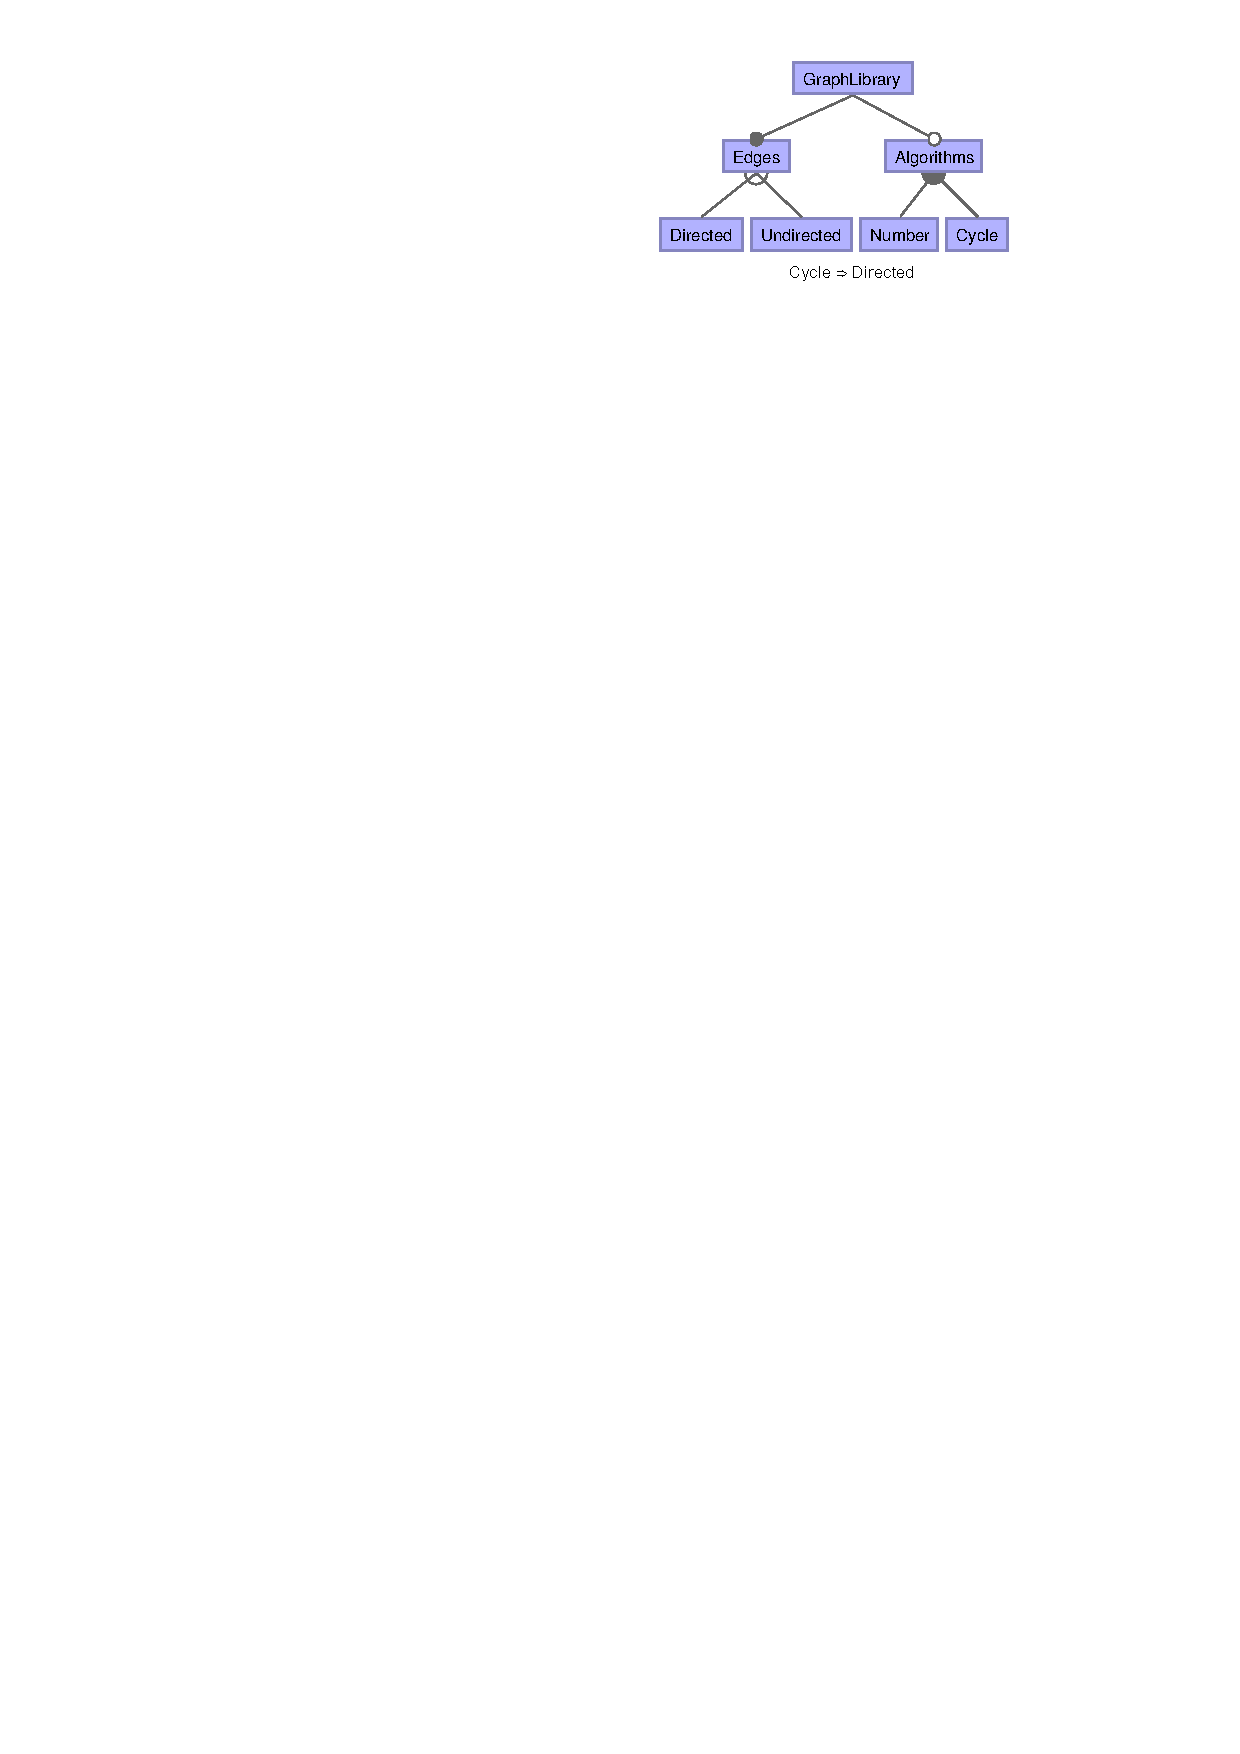
\includegraphics[scale=1.25]{example}
	\caption{A feature model representing a graph product line}
	\label{fig:ex}
\end{figure}

\section{Tables}

\vref{tab:ex} shows the result of a simple tabular environment.

\begin{table}[htbp]
	\centering
		\begin{tabular}{cc} \toprule
			Group Type & Propositional Formula\\ \midrule
			And & $(P \pimplies C_{k_1} \wedge\ldots\wedge C_{k_m}) \pand (C_1\vee\ldots\vee C_n \pimplies P)$\\\addlinespace
			Or & $P \pequals C_1\vee\ldots\vee C_n$\\ \addlinespace
			Alternative & $(P \pequals C_1\vee\ldots\vee C_n) \pand \mbox{atmost}1(C_1,\ldots,C_n)$\\
			\bottomrule
		\end{tabular}
	\caption{Mapping a feature model to a propositional formula}
	\label{tab:ex}
\end{table}

\section{Code Listings}

In \vref{lst:ex}, we give an example of a source code listing. 

\begin{lstlisting}[style=Java,float=htb,caption={Java source code},label={lst:ex}]
class A extends Object {
	A() { super(); }
}
class B extends Object {
	B() { super(); }
}
class Pair extends Object {
	Object fst;
	Object snd;
	Pair(Object fst, Object snd) {
		super(); this.fst=fst; this.snd=snd;
	}
	Pair setfst(Object newfst) {
		return new Pair(newfst, this.snd);
	}
}
\end{lstlisting}

% concrete solution of your problem (tooling, algorithms, etc.)
\chapter{Implementation}
\label{ch:Implementation}
%% ==============================
\hint{Most theses in computer science are accompanied by tool support written by the author of the thesis. Such tools enable an empirical evaluation or simply serve as a proof-of-concept. In particular, tools are typically not the ultimate goal in research, but often necessary to evaluate whether proposed concepts solve real problems. Hence, it is common to write about the tool in a dedicated chapter.}

\hint{The tool chapter has several goals. For supervisors, it typically helps to estimate the implementation effort of a thesis and problems faced during development. For other students, the chapter serves as the documentation of the tool support. That is, students that extend the tool support will use this chapter to get an overview on the architecture and learn from failed attempts. As researchers are typically rather interested in concepts or evaluations, this dedicated chapter on tool support helps to remove clutter from other chapters. Nevertheless, researchers may be interested to read why tool support has been build the way it is and why it is build on certain existing tools or libraries. Write the chapter such that it useful for researchers, students, and supervisors.}

\todots
    
% the evaluation of your work (planning, design, execution, results, discussion)
\chapter{Evaluation}
\label{ch:Evaluation}
%% ==============================
%The assessment is one of the most important sections of the work
%- It contains the quintessence of the whole project
%Many people only read the introduction and the assessment
%- So everything important must be in here!
%Here you prove that you ...
%- understood the task and its meaning
%- are able to interpret the results correctly
%- know what was important in this work

\todots
 
% describe research related to your own work and differentiate between your concept and existing approaches
\chapter{Related Work}
\label{ch:relatedWork}

\todots

% Summary of your work and its results.
% Includes a discussion about future work and how to procede with our results
\chapter{Conclusion and Outlook}
\label{ch:Conclusion}
%% ==============================
\hint{Summarize the contribution of the entire work and highlight the importance of the results}

\hint{Outlook on further development of the results}

\hint{(No more subsections!)}

\todots 

%% ++++++++++++++++++++++++++++++++++++++++++
%% Literature
%% ++++++++++++++++++++++++++++++++++++++++++
%  with the command \nocite also non cited references are also printed
\cleardoublepage
\phantomsection
\addcontentsline{toc}{chapter}{\bibname}
%%
% only specify if sources not cited in the text are also to appear
\nocite{*} 
%########## different citation styles
% with abbreviated first names of the authors
% abbrvnat unsrtnat
%\bibliographystyle{gerplain}
\bibliographystyle{alpha}
\bibliography{literature/bibAbrv, literature/bibFull, literature/literature}

%% ++++++++++++++++++++++++++++++++++++++++++
%% apendix
%% ++++++++++++++++++++++++++++++++++++++++++

\appendix
%% Here you place content you produced, which take to much space in your thesis
%% It is not mandatory to have appendix material, but most of the time you have some assets you do not want to show in your thesis directly
\chapter{Appendix}
Appendix

\end{document}
%% end of file
